\documentclass[12pt,AutoFakeBold]{article} 

\usepackage[微机原理与系统设计]{XDULabreport}  % 载入 XDULabreport 模板文件,[]中填写科目名称,科目名称,默认为电子线路实验(I)
\problem{第四章上机习题}  % 请在此处填写问题内容
\coauthor{} % 同作者姓名
\labdate{2021年10月20日} % 实验日期
% 其他参数在宏包中进行更改,其中学院,班级,姓名,学号均在sty宏包内进行更改
% \usepackage{fourier}  % 这是 fourier 字体,更柔和 

\newfontfamily\digi{DigifaceWide Regular} % 将数码管字体引入

%% 如果你需要中文的一级标题编号,如“一、”、“二、”等,请把下面两行取消注释
% \RequirePackage{zhnumber} % change section number to chinese
% \titleformat{\section}{\Large\bfseries\rmfamily}{\zhnum{section}、}{0em}{}

% 文档开始
        
\begin{document}

\maketitle
\setcounter{tocdepth}{2}
\tableofcontents  % 生成目录


% 正文标题
\makeatletter
\begin{center}
    \LARGE \textbf{\textsf{\@problem}}
\end{center}
\makeatother

% 正文开始




\section{实验目的}

完成第四章习题里的两个上机题目,如下

\begin{itemize}
	\item [4.47] 用同余法产生 200 个小于 256 的伪随机数,统计其中奇数的个数,并计算所有奇数的和,将奇数个数存入名为 \lstinline|CNT| 的字节单元,和存入名为 \lstinline|SUMODD| 的字存储单元中。用完整的段定义语句编写出实现这一功能的汇编语言源程序。
	\item [4.53] 设有 $n$ (设为 17) 个人围坐在圆桌周围,按顺时针给他们编号($1,2,\cdots,n$),从第 1 个人开始顺时针方向加 1 报数,当报数到 $m$ (设为 11) 时,该人出列,余下的人继续进行,直到所有人出列。编写程序模拟这一过程,求出出列人的编号顺序。
\end{itemize}


\section{实验环境}

\begin{itemize}
	\item emu8086: 编写汇编语言程序,并进行编译和连接,生成一个可执行程序
	\item \LaTeX: 制作封面并进行文档编写排版
	\item Visio 2016: 程序相关流程图绘制
\end{itemize}

\section{方案设计}

\subsection{题目 4.47 设计方案}

设计的产生伪随机数的递归公式为
%
\begin{equation*}
X_{i+1}\equiv5X_i+3\quad\pmod {256}
\end{equation*}
%
题目 4.47 设计的流程图如图 \ref{pro:out1} 所示

\begin{figure}[hbtp]
	\centering
	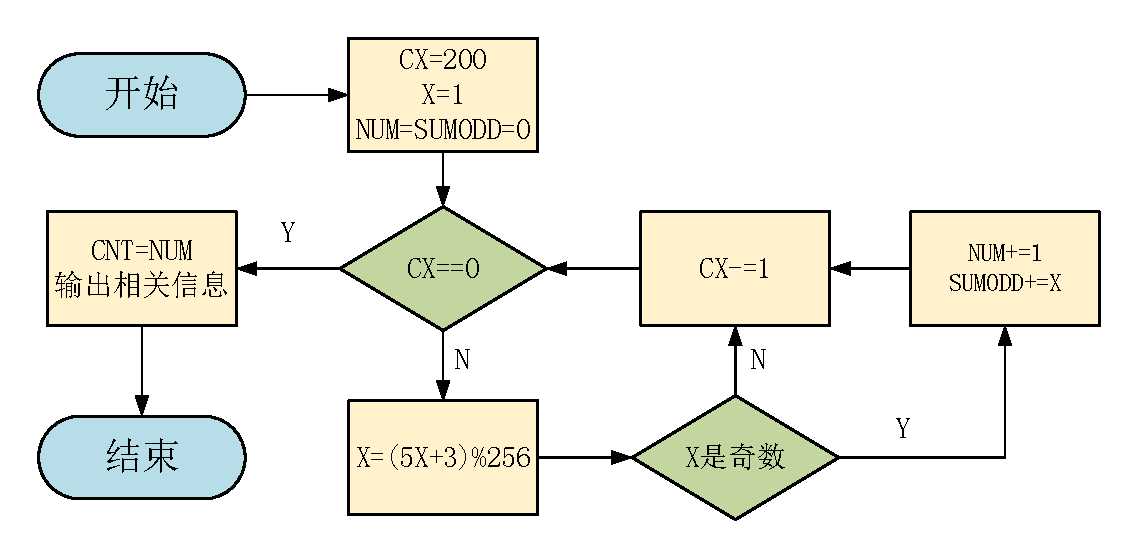
\includegraphics[width=16cm]{out1.pdf}
	\caption{题目 4.47 设计流程图}\label{pro:out1}
\end{figure}

\subsection{题目 4.53 设计方案}

题目 4.53 设计的流程图如图 \ref{pro:out2} 所示

\begin{figure}[hbtp]
	\centering
	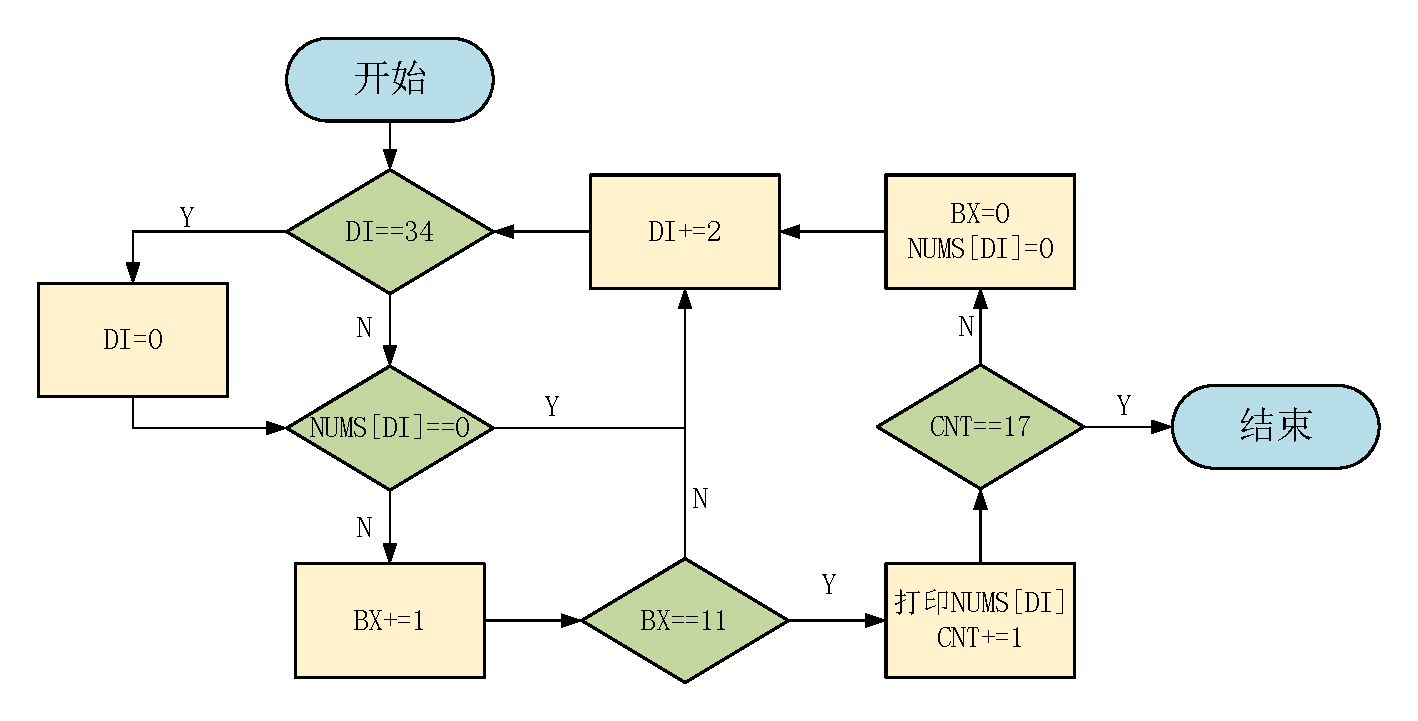
\includegraphics[width=16cm]{out2.pdf}
	\caption{题目 4.53 设计流程图}\label{pro:out2}
\end{figure}

\section{实验结果与分析}

题目 4.47 的输出结果显示,产生了 100 个奇数,它们的和是 13256,如图 \ref{fig:out1} 所示。

\begin{figure}[hbtp]
	\centering
	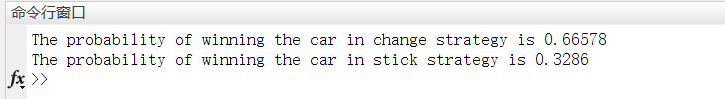
\includegraphics[width=16cm]{out1.png}
	\caption{题目 4.47 实验结果图}\label{fig:out1}
\end{figure}

题目 4.53 的输出结果显示,出列人的编号顺序为 11,5,17,13,9,7,6,8,12,16,4,2,3,15,10,14,1,如图 \ref{fig:out2} 所示。

\begin{figure}[hbtp]
	\centering
	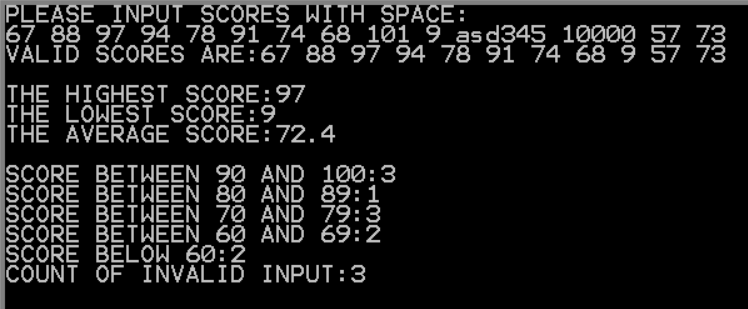
\includegraphics[width=16cm]{out2.png}
	\caption{题目 4.53 实验结果图}\label{fig:out2}
\end{figure}

\section{实验的收获及心得}

通过本次实验,我掌握了同余法生成伪随机数的方法和约瑟夫问题的汇编语言解法,提高了汇编语言程序设计技巧,能够较好地将思路转化为流程图,进一步熟悉了 \LaTeX 排版和 Viso 绘图技巧。但本次实验中的不足是,我虽然能够想到时间复杂度更低的算法,但由于汇编语言里不好实现一些数据结构而难以将其实现。

\section{实验代码}

\subsection{题目 4.47 代码}

\begin{lstlisting}[language={[x86masm]Assembler}]
DATA SEGMENT
	STR1 DB 'COUNT OF ODD NUMBERS:','$'
	STR2 DB 13,10,'SUM OF ODD NUMBERS:','$'
	STR0 DB 13,10,'$'
	CNT DW 0
	SUMODD DW 0
	NUM DW 0
	X DW 1
	A DW 5
	B DW 3
	MOD DW 256
DATA ENDS

STACK SEGMENT STACK 'STACK'
	DW 100H DUP(?)
STACK ENDS

CODE SEGMENT
	ASSUME CS:CODE,DS:DATA,SS:STACK
START:
	MOV AX, DATA 
	MOV DS, AX
	MOV AX, STACK
	MOV SS, AX
	MOV CX, 200

FOR1:
	MOV AX, X
	MUL A
	ADD AX, B
	DIV MOD
	MOV AX, DX ; (A*X+B)%MOD, A=5, B=3, MOD=256
	MOV X, AX
	SHR AX, 1
	JNC EVEN
	RCL AX, 1
	INC NUM
	ADD SUMODD, AX
	; LEA SI, X
	; CALL PRINT
	; MOV DX, OFFSET STR0
	; MOV AH, 9
	; INT 21H
EVEN:    
	LOOP FOR1    

	MOV DX, OFFSET STR1
	MOV AH, 9
	INT 21H
	LEA SI, NUM
	CALL PRINT
	MOV AL, BYTE PTR NUM
	MOV CNT, AL

	MOV DX, OFFSET STR2
	MOV AH,9
	INT 21H
	LEA SI, SUMODD
	CALL PRINT

	MOV AH, 4CH
	INT 21H

PRINT PROC NEAR
	PUSH AX
	PUSH BX
	PUSH CX
	PUSH DX

	MOV AX, [SI]
	MOV BX, 10
	MOV CX, 0
INIT:
	XOR DX, DX
	DIV BX ; 商 AX 余 DX
	INC CX
	PUSH DX
	CMP AX, 0
	JNZ INIT
OUTPUT:
	POP DX
	OR DX, 30H
	MOV AH, 2
	INT 21H
	LOOP OUTPUT

	POP DX
	POP CX
	POP BX
	POP AX
	RET
PRINT ENDP

CODE ENDS
END START
\end{lstlisting}

\subsection{题目 4.53 代码}

\begin{lstlisting}[language={[x86masm]Assembler}]
DATA SEGMENT
	NUMS DW 1, 2, 3, 4, 5, 6, 7, 8, 9, 10, 11, 12, 13, 14, 15, 16, 17, 0
	STR DB 'THE ORDER OF QUEUE IS:',13,10,'$'
	CNT DW 0
DATA ENDS

STACK SEGMENT STACK 'STACK'
	DW 100H DUP(?)    
STACK ENDS

CODE SEGMENT
	ASSUME CS:CODE, DS:DATA, SS:STACK
START:
	MOV AX, DATA
	MOV DS, AX
	MOV AX, STACK
	MOV SS, AX

	XOR BX, BX ; 当前报的数
	XOR SI, SI
	XOR DI, DI

	MOV DX, OFFSET STR
	MOV AH, 9
	INT 21H

L0:    
	CMP DI, 34
	JNZ L1
	XOR DI, DI
L1:
	CMP NUMS[DI], 0
	JNZ L2
	ADD DI, 2
	JMP L0
L2:
	INC BX
	CMP BX, 11
	JZ OK
	ADD DI, 2
	JMP L0
OK: 
	PUSH SI ; 打印出列顺序                
	LEA SI, NUMS[DI]
	CALL PRINT
	MOV DL, 32
	MOV AH, 2
	INT 21H
	POP SI

	INC CNT
	CMP CNT, 17
	JZ OVER
	XOR BX, BX ; 报数清0
	MOV NUMS[DI], 0
	ADD DI, 2
	JMP L0    
OVER:

	MOV AH, 4CH
	INT 21H 

PRINT PROC NEAR
	PUSH AX
	PUSH BX
	PUSH CX
	PUSH DX

	MOV AX, [SI]
	MOV BX, 10
	MOV CX, 0
INIT:
	XOR DX, DX
	DIV BX ; 商 AX 余 DX
	INC CX
	PUSH DX
	CMP AX, 0
	JNZ INIT
OUTPUT:
	POP DX
	OR DX, 30H
	MOV AH, 2
	INT 21H
	LOOP OUTPUT

	POP DX
	POP CX
	POP BX
	POP AX
	RET
PRINT ENDP

CODE ENDS
END START
\end{lstlisting}

% % 参考文献,此处以 MLA 引用格式为例

%\begin{thebibliography}{9}
%\end{thebibliography}

% % \includepdf[pages={1,2}]{Memo.pdf} 
% 可以直接导入pdf页面
%\newpage
%\begin{appendices}  % 附录环境
%\section{核心层}\label{subsec:B}
%\end{appendices}
\end{document}  % 结束